\documentclass[12pt]{article}
\usepackage{amsthm,amssymb,amsfonts,amsmath,amstext,systeme,adjustbox}
\usepackage{graphicx,float,wrapfig}
\usepackage{tabularx,enumitem}
\graphicspath{{PPFigure/}}
\marginparwidth 0pt
\oddsidemargin -1.2 truecm
\evensidemargin  0pt 
\marginparsep 0pt
\topmargin -2.2truecm
\linespread{1}
\textheight 25.8 truecm
\textwidth 18.5 truecm
\newenvironment{remark}{\noindent{\bf Remark }}{\vspace{0mm}}
\newenvironment{remarks}{\noindent{\bf Remarks }}{\vspace{0mm}}
\newenvironment{question}{\noindent{\bf Question }}{\vspace{0mm}}
\newenvironment{questions}{\noindent{\bf Questions }}{\vspace{0mm}}
\newenvironment{note}{\noindent{\bf Note }}{\vspace{0mm}}
\newenvironment{summary}{\noindent{\bf Summary }}{\vspace{0mm}}
\newenvironment{back}{\noindent{\bf Background}}{\vspace{0mm}}
\newenvironment{conclude}{\noindent{\bf Conclusion}}{\vspace{0mm}}
\newenvironment{concludes}{\noindent{\bf Conclusions}}{\vspace{0mm}}
\newenvironment{dill}{\noindent{\bf Description of Dill's model}}{\vspace{0mm}}
\newenvironment{maths}{\noindent{\bf Mathematics needed}}{\vspace{0mm}}
\newenvironment{inst}{\noindent{\bf Instructions}}{\vspace{0mm}}
\newenvironment{notes}{\noindent{\bf Notes }}{\vspace{0mm}}
\newenvironment{theorem}{\noindent{\bf Theorem }}{\vspace{0mm}}
\newenvironment{example}{\noindent{\bf Example }}{\vspace{0mm}}
\newenvironment{examples}{\noindent{\bf Examples }}{\vspace{0mm}}
\newenvironment{topics}{\noindent{\bf Topics}}{\vspace{0mm}}
\newenvironment{outcomes}{\noindent{\bf Expected Learning Outcomes}}{\vspace{0mm}}
\newenvironment{lemma}{\noindent{\bf Lemma }}{\vspace{0mm}}
\newenvironment{solution}{\noindent{\it Solution}}{\vspace{2mm}}
\newcommand{\ds}{\displaystyle}
\newcommand{\un}{\underline}
\newcommand{\bs}{\boldsymbol}

\begin{document}

\baselineskip 18 pt
\begin{center}
	{\large \bf HKDSE MATH Core Practice Paper II}\\
	\vspace{2 mm}
\end{center}
\vspace{0.05cm}

\begin{enumerate}
	\item \textbf{HKDSE MATH Core Practice Paper II Q1}\\
	$x^3(2x + x) = $
	\begin{enumerate}
		\item[A.] $3x^4$.
		\item[B.] $2x^5$.
		\item[C.] $3x^5$.
		\item[D.] $2x^6$.
	\end{enumerate}

	\item \textbf{HKDSE MATH Core Practice Paper II Q2}\\
	If $3a + 1 = 3(b - 2)$, then $b =$
	\begin{enumerate}
		\item[A.] $a + 1$.
		\item[B.] $a + 3$.
		\item[C.] $a + \dfrac{7}{3}$.
		\item[D.] $a - \dfrac{5}{3}$.
	\end{enumerate}

	\item \textbf{HKDSE MATH Core Practice Paper II Q3}\\
	$p^2 - q^2 - p - q =$
	\begin{enumerate}
		\item[A.] $(p + q)(p - q - 1)$.
		\item[B.] $(p + q)(p + q - 1)$.
		\item[C.] $(p - q)(p - q + 1)$.
		\item[D.] $(p - q)(p + q - 1)$.
	\end{enumerate}

	\item \textbf{HKDSE MATH Core Practice Paper II Q4}\\
	Let $m$ and $n$ be constants. If $m(x - 3)^2 + n(x + 1)^2 \equiv x^2 - 38x + 41$, then $m = $
	\begin{enumerate}
		\item[A.] $-4$.
		\item[B.] $-1$.
		\item[C.] $3$.
		\item[D.] $5$.
	\end{enumerate}

	\item \textbf{HKDSE MATH Core Practice Paper II Q5}\\
	Let $f(x) = x^4 - x^3 + x^2 - x + 1$. When $f(x)$ is divided by $x + 2$, the remainder is 
	\begin{enumerate}
		\item[A.] $-2$.
		\item[B.] $0$.
		\item[C.] $11$.
		\item[D.] $31$.
	\end{enumerate}

	\item \textbf{HKDSE MATH Core Practice Paper II Q6}\\
	Let $k$ be a constant. If the quadratic equation $3x^2 + 2kx - k = 0$ has equal roots, then $k = $
	\begin{enumerate}
		\item[A.] $-3$.
		\item[B.] $3$.
		\item[C.] $-3$ or $0$.
		\item[D.] $0$ or $3$.
	\end{enumerate}

	\item \textbf{HKDSE MATH Core Practice Paper II Q7}\\
	In the figure, the $x$-intercept of the straight lines $L_1$ and $L_2$ are 5 while the $y$-intercepts of the straight lines $L_2$ and $L_3$ are 3. Which og the following are true?
	\begin{enumerate}
		\item[I.] The solution of the inequality $f(x) > k$ is $x < 1$ or $x > 7$.
		\item[II.] The roots of the equation $f(x) = k$ are 1 and 7.
		\item[III.] The equation of the axis of symmetry of the quadratic graph of $y = f(x)$ is $x = 3$.
		\item[]
			\begin{minipage}[u]{.39\textwidth}
				\begin{enumerate}
					\item[A.] I and II only
					\item[B.] I and III only
					\item[C.] II and III only
					\item[D.] I, II and III
				\end{enumerate}
			\end{minipage}
			\begin{minipage}[u]{.5\textwidth}
				\centering
				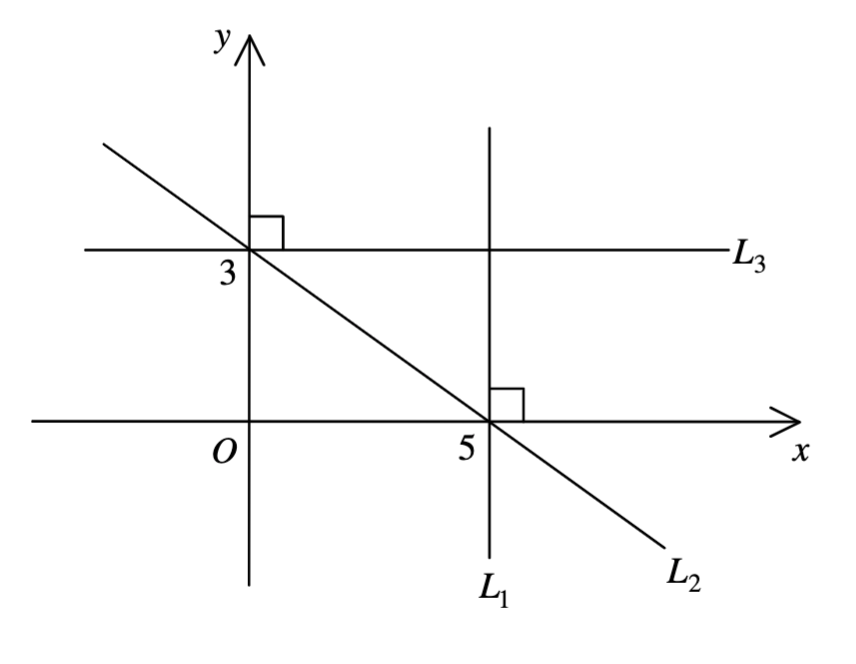
\includegraphics[scale=0.6]{PPFigure2.7.png}
			\end{minipage}
	\end{enumerate}

	\item \textbf{HKDSE MATH Core Practice Paper II Q8}\\
	The figure shows the graph of $y = ax^2 - 2x + b$, where $a$ and $b$ are constants. Which of the following is/are true?
	\begin{enumerate}
		\item[I.] $a > 0$
		\item[II.] $b < 0$
		\item[III.] $ab < 1$
		\item[]
			\begin{minipage}[u]{.39\textwidth}
				\begin{enumerate}
					\item[A.] I only
					\item[B.] II only
					\item[C.] I and III only
					\item[D.] II and III only
				\end{enumerate}
			\end{minipage}
			\begin{minipage}[u]{.5\textwidth}
				\centering
				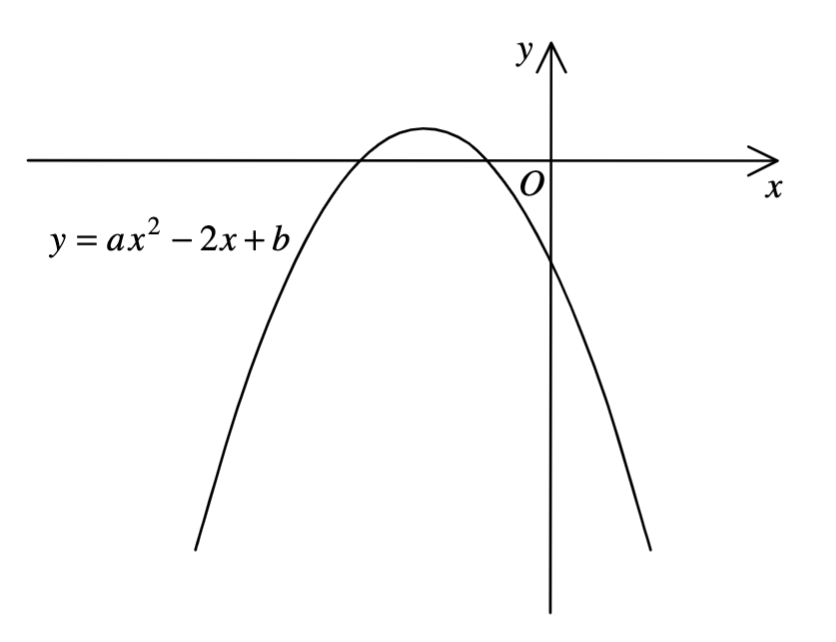
\includegraphics[scale=0.6]{PPFigure2.8.png}
			\end{minipage}
	\end{enumerate}
		
	\item \textbf{HKDSE MATH Core Practice Paper II Q9}\\
	The solution of $4x > x - 3$ or $3 - x < x + 7$ is
	\begin{enumerate}
		\item[A.] $x > -2$.
		\item[B.] $x < -2$.
		\item[C.] $x > -1$
		\item[D.] $x < -2$ or $x > -1$.
	\end{enumerate}

	\item \textbf{HKDSE MATH Core Practice Paper II Q10}\\
	John buys a vase for \$1600. He then seels the vase to Susan at a profit of 20\%. At what price should Susan sell the vase in order to have a profit of 20\%?
	\begin{enumerate}
		\item[A.] \$2240
		\item[B.] \$2304
		\item[C.] \$2400
		\item[D.] \$2500
	\end{enumerate}

	\item \textbf{HKDSE MATH Core Practice Paper II Q11}\\
	If the circumference of a circle is increased by 40\%, then the area of the circle is increased by	
	\begin{enumerate}
		\item[A.] 18\%.
		\item[B.] 20\%.
		\item[C.] 40\%.
		\item[D.] 96\%.
	\end{enumerate}

	\item \textbf{HKDSE MATH Core Practice Paper II Q12}\\
	Let $\alpha$ and $\beta$ be non-zero constants. If $(\alpha + \beta) : (3\alpha - \beta) = 7 : 3$, then $\alpha : \beta = $
	\begin{enumerate}
		\item[A.] $5 : 9$.
		\item[B.] $9 : 5$.
		\item[C.] $19 : 29$.
		\item[D.] $29 : 19$.
	\end{enumerate}

	\item \textbf{HKDSE MATH Core Practice Paper II Q13}\\
	If $z$ varies directly as $x$ and inversely as $y^2$, which of the folowing must be constant?
	\begin{enumerate}
		\item[A.] $\dfrac{x}{y^2z}$
		\item[B.] $\dfrac{z}{xy^2}$
		\item[C.] $\dfrac{yz}{x^2}$
		\item[D.] $\dfrac{xz}{y^2}$
	\end{enumerate}

	\item \textbf{HKDSE MATH Core Practice Paper II Q14}\\
	$0.009049999 =$
	\begin{enumerate}
		\item[A.] 0.00905 (correct to 3 decimal places).
		\item[B.] 0.00905 (correct to 3 significant figures).
		\item[C.] 0.00905 (correct to 6 decimal places).
		\item[D.] 0.00905 (correct to 6 significant figures).
	\end{enumerate}

	\item \textbf{HKDSE MATH Core Practice Paper II Q15}\\
	In the figure, $O$ is the centre of the sector $OABC$. If the area of $\triangle OAC$ is 12 cm$^2$, find the area of the segment $ABC$.
	\begin{figure}[H]
		\centering
		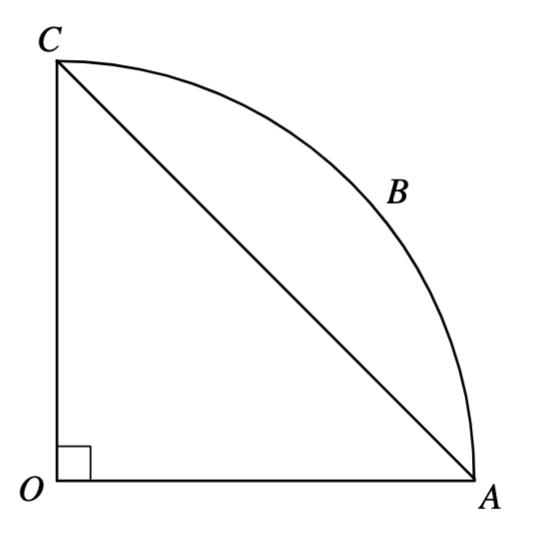
\includegraphics[width = 0.8\textwidth]{PPFigure2.15}
	\end{figure}
	\begin{enumerate}
		\item[A.] $3(\pi - 2)$ cm$^2$
		\item[B.] $3(\pi - 1)$ cm$^2$
		\item[C.] $6(\pi - 2)$ cm$^2$
		\item[D.] $6(\pi - 1)$ cm$^2$
	\end{enumerate}

	\item \textbf{HKDSE MATH Core Practice Paper II Q16}\\
	The figure shows a right circular cone of height 8 cm and slant height 17 cm. Find the volume of the circular cone.
	\begin{figure}[h]
		\centering
		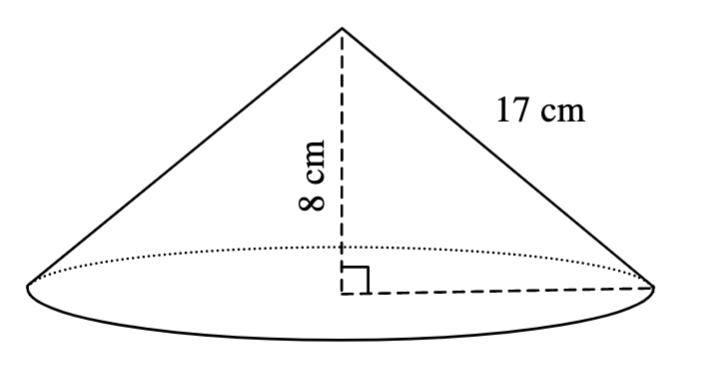
\includegraphics[width = 0.3\textwidth]{PPFigure2.16.png}	
	\end{figure}
	\begin{enumerate}
		\item[A.] $225\pi$ cm$^3$
		\item[B.] $345\pi$ cm$^3$
		\item[C.] $480\pi$ cm$^3$
		\item[D.] $600\pi$ cm$^3$
	\end{enumerate}

	\item \textbf{HKDSE MATH Core Practice Paper II Q17}\\
	In the figure, $ABCD$ is a rectangular. $E$ is the mid-point of $BC$. $F$ is a point lying on $CD$ such that $DF = 2CF$. If the area of $\triangle CEF$ is 1 cm$^2$, then the area of $\triangle AEF$ is 
	\begin{figure}[H]
		\centering
		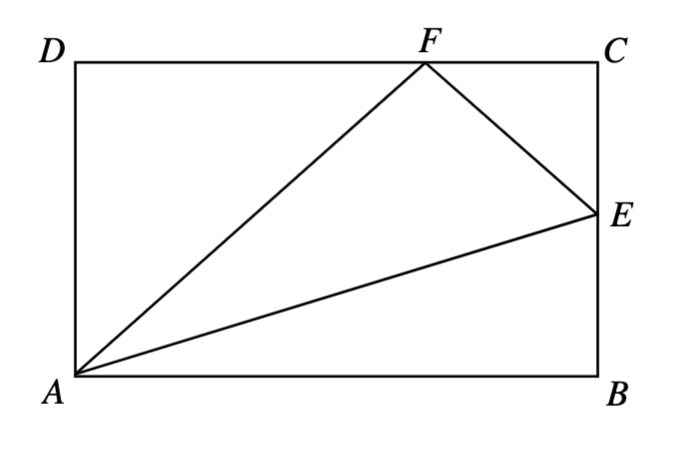
\includegraphics[width = 0.7\textwidth]{PPFigure2.17.png}	
	\end{figure}
	\begin{enumerate}
		\item[A.] 2 cm$^3$
		\item[B.] 3 cm$^3$
		\item[C.] 4 cm$^3$
		\item[D.] 6 cm$^3$
	\end{enumerate}

	\item \textbf{HKDSE MATH Core Practice Paper II Q18}\\
	In the figure, $AB = 4$ cm, $BC = CD = DE = 8$ cm and $FG = 9$ cm. Find the perimeter of $\triangle AEH$.
	\begin{figure}[H]
		\centering
		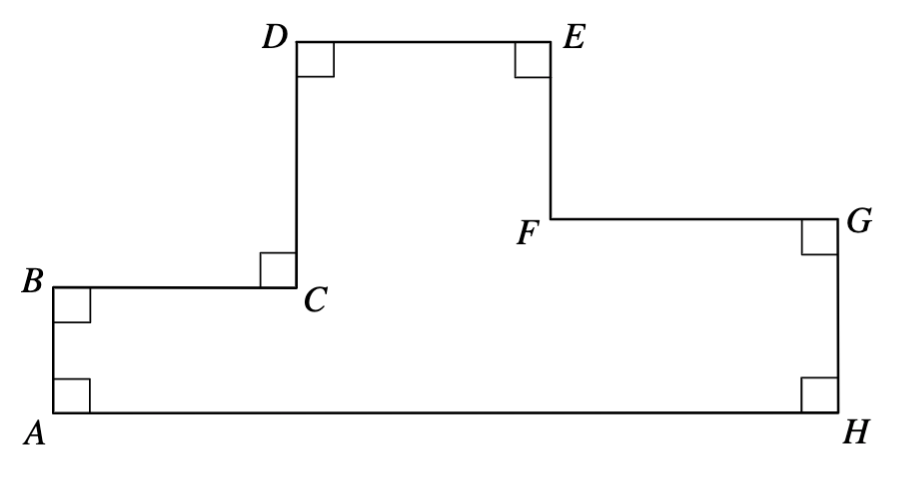
\includegraphics[width = 0.7\textwidth]{PPFigure2.18.png}	
	\end{figure}
	\begin{enumerate}
		\item[A.] 60 cm.
		\item[B.] 74 cm.
		\item[C.] 150 cm.
		\item[D.] 164 cm.
	\end{enumerate}

	\item \textbf{HKDSE MATH Core Practice Paper II Q19}\\
	In the figure, $AB = BC$ and $D$ is a point lying on $BC$ such that $CD = DE$. If $AB // CE$, find $\angle CDE$.
	\begin{enumerate}
		\item[A.] $ \sin{\theta}$.
		\item[B.] $3\sin{\theta}$.
		\item[C.] $2\sin{\theta} - \cos{\theta}$.
		\item[D.] $2\sin{\theta} + \cos{\theta}$.
	\end{enumerate}

	\item \textbf{HKDSE MATH Core Practice Paper II Q20}\\
	In the figure, $AB = 1$ cm, $BC = CD = DE = 2$ cm and $EF = 3$ cm. Find the distance between $A$ and $F$ correct to the nearest 0.1 cm.
	\begin{figure}[H]
		\centering
		\includegraphics[width = 0.7\textwidth]{PPFigure2.20.png}	
	\end{figure}
	\begin{enumerate}
		\item[A.] 7.2 cm
		\item[B.] 7.4 cm
		\item[C.] 8.0 cm
		\item[D.] 8.1 cm
	\end{enumerate}

	\item \textbf{HKDSE MATH Core Practice Paper II Q21}\\
	In the figure, $ABCD$ is a semi-circle. If $BC = CD$, then $\angle ADC = $
	\begin{figure}[H]
		\centering
		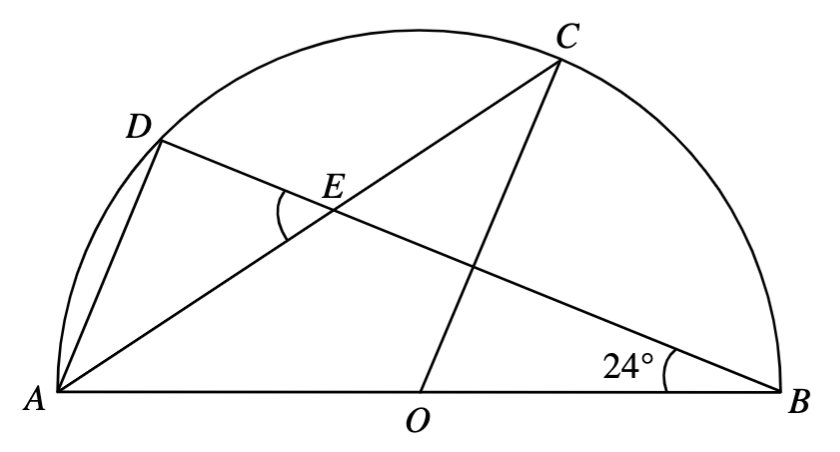
\includegraphics[width = 0.7\textwidth]{PPFigure2.21.png}	
	\end{figure}
	\begin{enumerate}
		\item[A.] 118$^\circ$.
		\item[B.] 121$^\circ$.
		\item[C.] 124$^\circ$.
		\item[D.] 126$^\circ$.
	\end{enumerate}

	\item \textbf{HKDSE MATH Core Practice Paper II Q22}\\
	In the figure, $O$ is the centre of the circle $ABCDE$. If $\angle ABE = 30^\circ$ and $\angle CDE = 105^\circ$, then $\angle AOC = $
	\begin{figure}[H]
		\centering
		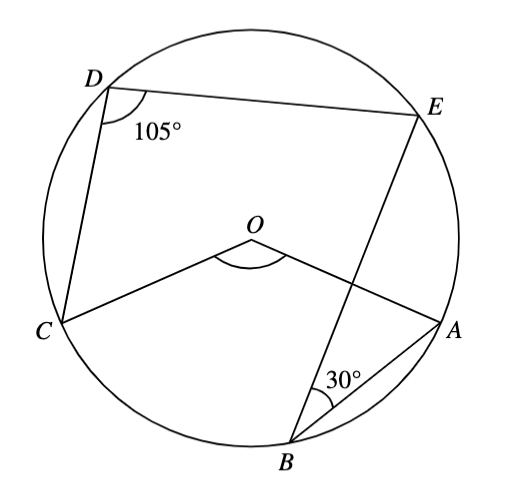
\includegraphics[width = 0.7\textwidth]{SPFigure2.22.png}	
	\end{figure}
	\begin{enumerate}
		\item[A.] 120$^\circ$.
		\item[B.] 135$^\circ$.
		\item[C.] 150$^\circ$.
		\item[D.] 165$^\circ$.
	\end{enumerate}
	
	\item \textbf{HKDSE MATH Core Practice Paper II Q23}\\
	In the figure, $ABCD$ is a parallelogram. $F$ is a point lying on $AD$. $BF$ produced and $CD$ produced meet at $E$ . If $CD : DE = 2 : 1$, then $AF : BC =$
	\begin{figure}[H]
		\centering
		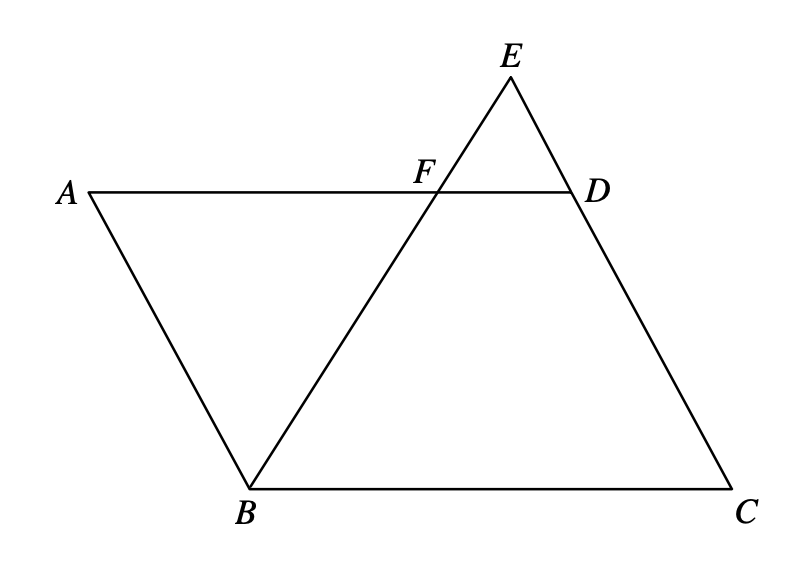
\includegraphics[width = 0.7\textwidth]{SPFigure2.23.png}	
	\end{figure}
	\begin{enumerate}
		\item[A.] $1 : 2$.
		\item[B.] $2 : 3$.
		\item[C.] $3 : 4$.
		\item[D.] $8 : 9$.
	\end{enumerate}

	\item \textbf{HKDSE MATH Core Practice Paper II Q24}\\
	In the figure, $ABC$ is a straight line. If $BD = CD$ and $AB = 10$ cm, find $BC$ corrent to the nearest cm.
	\begin{figure}[H]
		\centering
		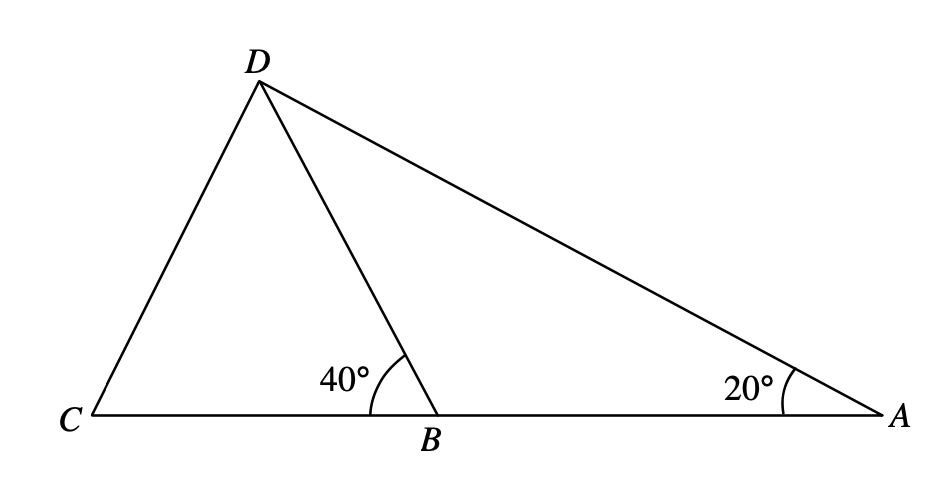
\includegraphics[width = 0.7\textwidth]{SPFigure2.24.png}	
	\end{figure}
	\begin{enumerate}
		\item[A.] 8 cm
		\item[B.] 13 cm
		\item[C.] 14 cm
		\item[D.] 15 cm
	\end{enumerate}

	\item \textbf{HKDSE MATH Core Practice Paper II Q25}\\
	In the figure, the two 6-sided polygons show
	\begin{figure}[H]
		\centering
		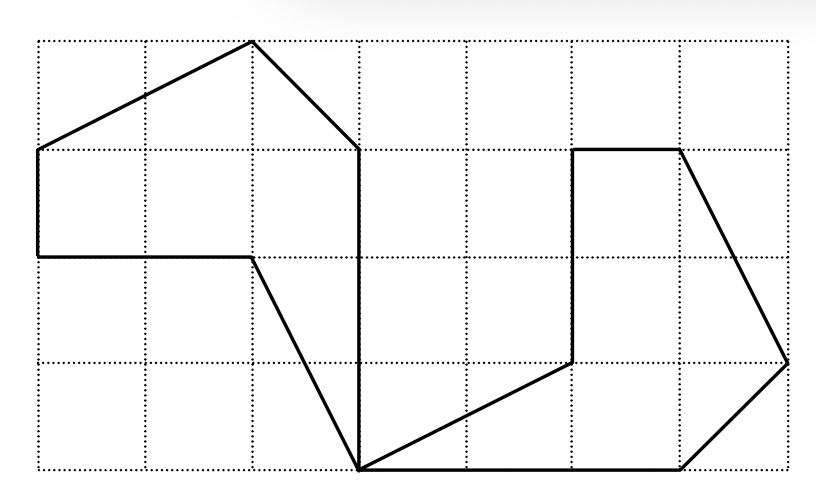
\includegraphics[width = 0.7\textwidth]{SPFigure2.25.png}	
	\end{figure}
	\begin{enumerate}
		\item[A.] a rotation transformation.
		\item[B.] a reflection transformation.
		\item[C.] a translation transformation.
		\item[D.] a dilation transformation.
	\end{enumerate}
	
	\item \textbf{HKDSE MATH Core Practice Paper II Q26}\\
	If the point $(-4, 3)$ is rotated anti-clockwise about the origin through $180^\circ$, then the coordinates of its image are
	\begin{enumerate}
		\item[A.] $(-3, -4)$.
		\item[B.] $(3, 4)$.
		\item[C.] $(-4, -3)$.
		\item[D.] $(4, -3)$.
	\end{enumerate}
	
	\item \textbf{HKDSE MATH Core Practice Paper II Q27}\\
	The box-and-whisker diagram below shows the distribution of the scores (in marks) of the students of a class in a test.
	\begin{figure}[H]
		\centering
		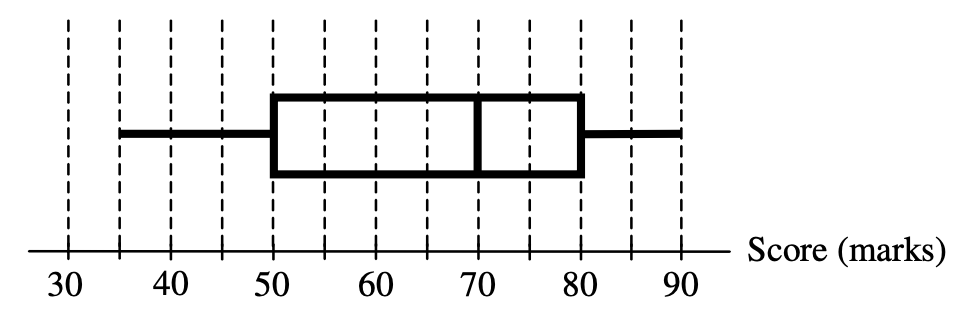
\includegraphics[width = 0.7\textwidth]{SPFigure2.27.png}	
	\end{figure}
	If the passing score of the test is 50 marks, then the passing percentage of the class is
	\begin{enumerate}
		\item[A.] 25\%.
		\item[B.] 50\%.
		\item[C.] 70\%.
		\item[D.] 75\%.
	\end{enumerate}
	
	\item \textbf{HKDSE MATH Core Practice Paper II Q28}\\
	The stem-and-leaf diagram below shows the distribution of heights (in cm) of 23 staff members in an office.
	\begin{table}[htbp]
		\centering
		\begin{tabular}{r|l@{\hspace{4 pt}}}
		    Stem (tens) & Leaf (units)\\
			\hline
			15     & 3 3 4 5 6 7 9\\    
			16     & 1 2 2 3 5 6 6 8\\    
			17     & 1 2 6 7 9\\
			18     & 2 6 7\\  
		\end{tabular}
		\label{tab:addlabel}
	\end{table}
	Find the median of the distribution.
	\begin{enumerate}
		\item[A.] 164 cm
		\item[B.] 165 cm
		\item[C.] 165.5 cm
		\item[D.] 166 cm
	\end{enumerate}
	
	\item \textbf{HKDSE MATH Core Practice Paper II Q29}\\
	$\{ a - 7 , a - 1 , a , a + 2 , a + 4 , a + 8 \}$ and $\{ a - 9 , a - 2 , a - 1 , a  +3 , a + 4 , a + 6 \}$ are two groups of numbers. Which of the following is/are true?
	\begin{enumerate}
		\item[I.] The two groups of numbers have the same mean.
		\item[II.] The two groups of numbers have the same median.
		\item[III.] The two groups of numbers have the same range.
		\item[]
		\begin{enumerate}
			\item[A.] I only
			\item[B.] II only
			\item[C.] I and III only
			\item[D.] II and III only
		\end{enumerate}
	\end{enumerate}
	
	\item \textbf{HKDSE MATH Core Practice Paper II Q30}\\
	The students' union of a school of 950 students wants to investigate the opinions of students in the school on the services provided by the tuck shop. A questionnaire is designed by the students' union and only the chairperson and vice-chairperson of the students' union are selected as a Practice to fill in the questionnaire. Which of the following are the disadvantages of this sampling method?
	\begin{enumerate}
		\item[I.] The Practice size is very small.
		\item[II.] Not all students in the school are selected.
		\item[III.] Not all students in the school have an equal chance of being selected.
		\item[]
		\begin{enumerate}
			\item[A.] I and II only
			\item[B.] I and III only
			\item[C.] II and III only
			\item[D.] I, II and III
		\end{enumerate}
	\end{enumerate}
	
	\item \textbf{HKDSE MATH Core Practice Paper II Q31}\\
	$\dfrac{1}{2 - x} + \dfrac{x - 1}{(x - 2)^2} = $
	\begin{enumerate}
		\item[A.] $\dfrac{-2}{(2 - x)^2}$.
		\item[B.] $\dfrac{1}{(2 - x)^2}$.
		\item[C.] $\dfrac{-2x + 3}{(2 - x)^2}$.
		\item[D.] $\dfrac{2x - 3}{(2 - x)^2}$.
	\end{enumerate}
	
	\item \textbf{HKDSE MATH Core Practice Paper II Q32}\\
	The graph in the figure shows the linear relation between $x$ and $\log_5{y}$. If $y = ab^x$, then $a =$
	\begin{figure}[H]
		\centering
		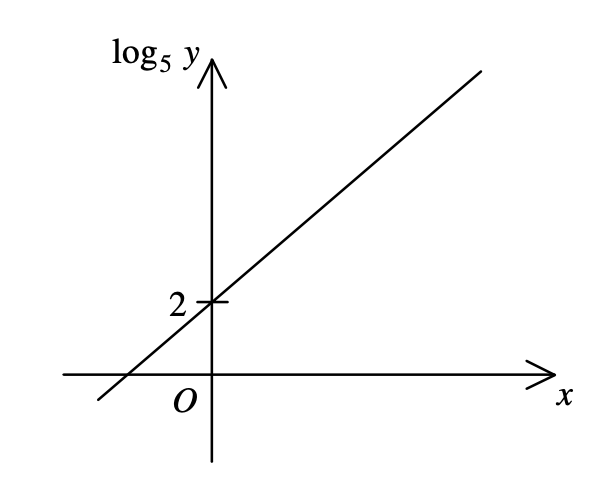
\includegraphics[width = 0.7\textwidth]{SPFigure2.32.png}	
	\end{figure}
	\begin{enumerate}
		\item[A.] 1.
		\item[B.] 2.
		\item[C.] 5.
		\item[D.] 25.
	\end{enumerate}
	
	\item \textbf{HKDSE MATH Core Practice Paper II Q33}\\
	$1010010001001_2 = $
	\begin{enumerate}
		\item[A.] $2^{12} + 2^{10} + 137$.
		\item[B.] $2^{12} + 2^{10} + 273$.
		\item[C.] $2^{13} + 2^{11} + 137$.
		\item[D.] $2^{13} + 2^{11} + 273$.
	\end{enumerate}
	
	\item \textbf{HKDSE MATH Core Practice Paper II Q34}\\
	If $k$ is a real number, then $4k - \dfrac{6 + ki}{i} = $
	\begin{enumerate}
		\item[A.] $3k + 6i$.
		\item[B.] $3k - 6i$.
		\item[C.] $5k + 6i$.
		\item[D.] $5k - 6i$.
	\end{enumerate}
	
	\item \textbf{HKDSE MATH Core Practice Paper II Q35}\\
	Which of the triangular regions in the figure may represent the solution of $\left\{
		\begin{matrix}
			0 \leq x \leq 6\\
			0 \leq y \leq 3\\
			x \leq 2y\\
		\end{matrix}\right.$?
	\begin{enumerate}
		\item[A.] $\triangle OAC$
		\item[B.] $\triangle OBD$
		\item[C.] $\triangle OCE$
		\item[D.] $\triangle ODF$
	\end{enumerate}
	
	\item \textbf{HKDSE MATH Core Practice Paper II Q36}\\
	If the 3rd term and the 6th term of an arithmetic sequence are 18 and $-6$ respectively, then 2nd term of the sequence is
	\begin{enumerate}
		\item[A.] $-8$.
		\item[B.] $10$.
		\item[C.] $26$.
		\item[D.] $34$.
	\end{enumerate}
	
	\item \textbf{HKDSE MATH Core Practice Paper II Q37}\\
	If the figure shows the graph of $y = f(x)$ and the graph of $y = g(x)$ on the same rectangular coordinate system, then
	\begin{figure}[H]
		\centering
		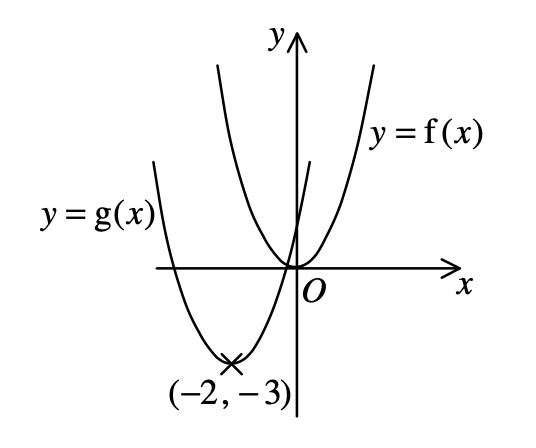
\includegraphics[width = 0.7\textwidth]{SPFigure2.37.png}	
	\end{figure}
	\begin{enumerate}
		\item[A.] $g(x) = f(x - 2) - 3$.
		\item[B.] $g(x) = f(x - 2) + 3$.
		\item[C.] $g(x) = f(x + 2) - 3$.
		\item[D.] $g(x) = f(x + 2) + 3$.
	\end{enumerate}
	
	\item \textbf{HKDSE MATH Core Practice Paper II Q38}\\
	In the figure, $y = $
	\begin{figure}[H]
		\centering
		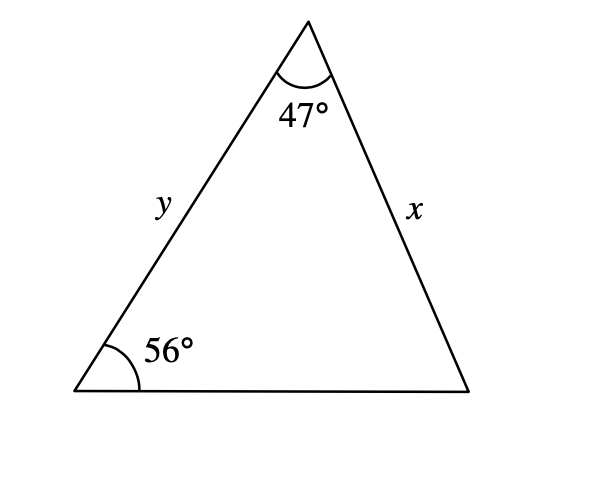
\includegraphics[width = 0.7\textwidth]{SPFigure2.38.png}	
	\end{figure}
	\begin{enumerate}
		\item[A.] $\dfrac{x\sin{77^\circ}}{\sin{56^\circ}}$.
		\item[B.] $\dfrac{x\sin{47^\circ}}{\sin{56^\circ}}$.
		\item[C.] $\dfrac{x\sin{56^\circ}}{\sin{77^\circ}}$.
		\item[D.] $\dfrac{x\sin{77^\circ}}{\sin{47^\circ}}$.
	\end{enumerate}
	
	\item \textbf{HKDSE MATH Core Practice Paper II Q39}\\
	Peter invests \$ $P$ at the beginning of each month in a year at an interest rate of 6\% per annum, compounded monthly. If he gets \$10 000 at the end of the year, find $P$ correct to the 2 decimal places.
	\begin{enumerate}
		\item[A.] 806.63
		\item[B.] 829.19
		\item[C.] 833.33
		\item[D.] 882.18
	\end{enumerate}
	
	\item \textbf{HKDSE MATH Core Practice Paper II Q40}\\
	The figure shows a cuboid $ABCDEFGH$. If the angle between the triangle $ACE$ and the plane $ABCD$ is $\theta$, then $\tan{\theta} = $
	\begin{figure}[H]
		\centering
		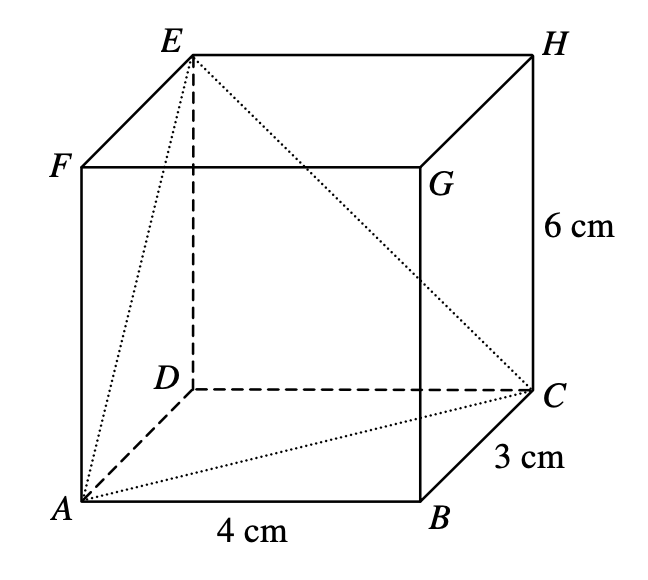
\includegraphics[width = 0.7\textwidth]{SPFigure2.40.png}	
	\end{figure}
	\begin{enumerate}
		\item[A.] 2.
		\item[B.] $\dfrac{3}{2}$.
		\item[C.] $\dfrac{5}{2}$.
		\item[D.] $\dfrac{12}{5}$.
	\end{enumerate}
	
	\item \textbf{HKDSE MATH Core Practice Paper II Q41}\\
	In the figure, $A$, $B$ and $C$ are points lying on the circle. $TA$ is the tangent to the circle at $A$. The straight line $CBT$ is perpendicular to $TA$. If $BC = 6$ cm, find the radius of the circle correct to the nearest 0.1 cm.
	\begin{figure}[H]
		\centering
		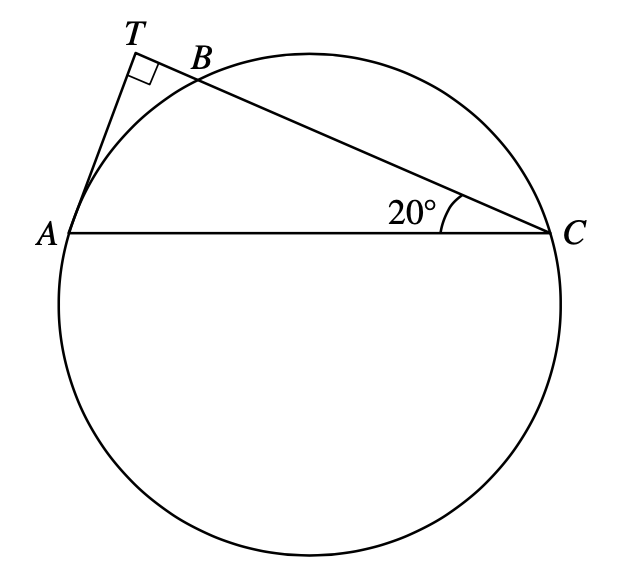
\includegraphics[width = 0.7\textwidth]{SPFigure2.41.png}	
	\end{figure}
	\begin{enumerate}
		\item[A.] 3.2 cm
		\item[B.] 3.9 cm
		\item[C.] 4.2 cm
		\item[D.] 4.7 cm
	\end{enumerate}
	
	\item \textbf{HKDSE MATH Core Practice Paper II Q42}\\
	Let $a$ be a constant and $-90^\circ < b < 90^\circ$. If the figure shows the graph of $y = a\cos{(x^\circ + b)}$, then 
	\begin{figure}[H]
		\centering
		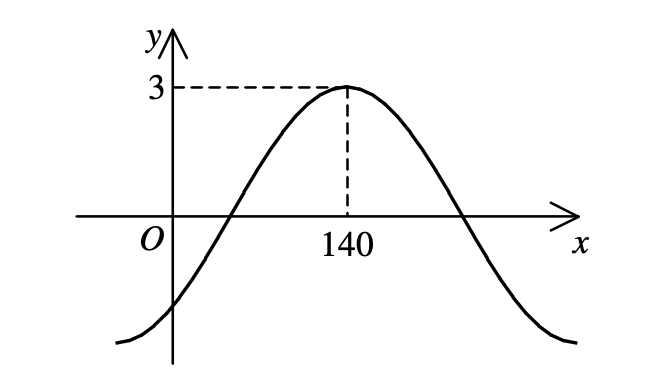
\includegraphics[width = 0.7\textwidth]{SPFigure2.42.png}	
	\end{figure}
	\begin{enumerate}
		\item[A.] $a = -3$ and $b = -40^\circ$.
		\item[B.] $a = -3$ and $b = 40^\circ$.
		\item[C.] $a = 3$ and $b = -40^\circ$.
		\item[D.] $a = 3$ and $b = 40^\circ$.
	\end{enumerate}
	
	\item \textbf{HKDSE MATH Core Practice Paper II Q43}\\
	Bag $A$ contains 2 red balls, 3 green balls and 4 white balls while bag $B$ contains 2 red balls, 3 green balls and 4 yellow balls. If one ball is drawn randomly from each bag, then the probability that the two balls drawn are of different colours is
	\begin{enumerate}
		\item[A.] $\dfrac{13}{81}$.
		\item[B.] $\dfrac{29}{81}$.
		\item[C.] $\dfrac{52}{81}$.
		\item[D.] $\dfrac{68}{81}$.
	\end{enumerate}
	
	\item \textbf{HKDSE MATH Core Practice Paper II Q44}\\
	If 2 girls and 5 boys randomly form a queue, find the probability that the two girls are next to each other in the queue.
	\begin{enumerate}
		\item[A.] $\dfrac{1}{7}$
		\item[B.] $\dfrac{2}{7}$
		\item[C.] $\dfrac{6}{7}$
		\item[D.] $\dfrac{1}{21}$
	\end{enumerate}
	
	\item \textbf{HKDSE MATH Core Practice Paper II Q45}\\
	A set of numbers has a mode of 32, an inter-quartile range of 27 and a variance of 25. If 3 is added to each number of the set and each resulting number is then doubled to form a new set of numbers, find the mode, the inter-quartile range and the variance of the new set of numbers.
	$\begin{matrix}
	&\text{Mode}&\text{Inter-quartile range}&\text{Variance}\\
	\text{A.}&64&60&50\\
	\text{B.}&70&60&100\\
	\text{C.}&70&54&50\\
	\text{D.}&70&54&100\\
	\end{matrix}$

\end{enumerate}
\end{document}

